\chapter{Teorema de Radó}

Finalmente estamos en condiciones de abordar el resultado principal de este Trabajo Fin de Grado, el teorema de Radó. Primero recordaremos  el concepto de superficie, seguiremos con el concepto de triangulación y por último el enunciado del teorema de Radó.

\begin{definition}
Una superficie $S \neq \emptyset$ es un espacio topológico que cumple que $\forall x \in S \exists V \subseteq S$ abierto con $x \in V$ y un homeomorfismo $\Phi : V \rightarrow U$ con $U$ un abierto de $\mathbb{R}^2$.A cada par $(V,\Phi)$ lo llamaremos carta local o sistema de coordenadas de $S$.
\end{definition}

\begin{remark}
Impondremos que $S$ sea Hausdorff y que cumpla el II Axioma de Numerabilidad.
\end{remark}

Consideremos ahora una colección $X$ de polígonos convexos dos a dos, junto con sus respectivos interiores, en el plano euclídeo tal que todas sus aristas son de longitud uno. Definamos un espacio topológico $S$ identificando cada arista de un polígono de $X$  con una  arista de otro, o del mismo, polígono. Está claro que el espacio identificación $S$, con la topología cociente inducida por la proyección natural $\pi\colon X\to S$,  es compacto. Además $S$ contiene de forma natural como subespacio el grafo $G$ con  vértices   la proyección de las esquinas de los polígonos de $X$ y como aristas la proyección de los lados de los polígonos de $X$.

\begin{lemma}
El espacio topológico $S$ anteriormente definido es una superficie si y sólo si $S$ es conexo y además es localmente homeomorfo a un disco en cada vértice de $G$.
\end{lemma}

\begin{definition}
En la situación anterior, diremos que el grafo $G$ es un embebimiento bicelular en $S$, es decir, que éste es un grafo embebido y además cada una de sus caras es homeomorfa a un disco abierto.
\end{definition}

\begin{definition}
Si todos los polígonos son triángulos, entonces decimos que $G$ es una triangulación de $S$ y que $S$ es una superficie triangulable.
\\
En el caso que estemos ante una triangulación tendremos que asumir que tenemos al menos cuatro triángulos (de otra forma $S$ no sería una superficie).
\end{definition}

Para la demostración del Teorema de Radó necesitaremos el siguiente resultado de Teoría de Grafos.
Este lema se podría haber encuadrado perfectamente en la sección que trataba sobre teoría básica de grafos, pero debido a que no se hace uso de él hasta este momento se ha ubicado en este apartado.

\begin{lemma}\label{lema27}
	Si $G$ es un grafo biconexo y $H$ es un subgrafo biconexo de $G$, entonces $G$ puede ser obtenido a partir de $H$ añadiendo caminos de forma sucesiva tal que cada uno de estos caminos una dos vértices distintos del grafo actual y el resto de vértices esté fuera del mismo.
\end{lemma}

\begin{proof}
	Haremos la demostración por inducción sobre el número de aristas de $E(G) \backslash E(H)$.

	Si ese número es cero, tenemos $G = H$. No hay nada que probar. Así que  asumamos que $G \neq H$. Por la hipótesis de inducción, el lema \ref{lema27} es válido cuando el par ($G,H$) es sustituido por otro par ($G',H'$) tal que $E(G') \backslash E(H')$ tiene menos aristas que $E(G) \backslash E(H)$. Ahora sea $H'$ un grafo biconexo maximal  de $G$ conteniendo a $H$. Si $H' \neq H$ aplicamos la hipótesis de inducción sobre ($H',H$) y entonces sobre ($G,H'$). Así que asumimos $H' = H$.

	Como $G$ es conexo, hay una arista $x_{1}x_{2}$ en $E(G) \backslash E(H)$ tal que $x_{1} \in H$. Como $G - x_{1}$ es conexo ($G$ es biconexo) existe un camino $P = x_{2}x_{3}...x_{k}$ tal que $x_{k} \in H$ y $X_i \notin H$ $\forall i = 2,... k-1$. Quizás $k = 2$. Ya que $H \cup P \cup {x_{1}x_{2}}$ es biconexo, tenemos que $G = H \cup P \cup {x_{1}x_{2}}$, lo que acaba la demostración.
\end{proof}

\begin{theorem}[\textbf{Teorema de Radó}]
	Toda superficie $S$ es homeomorfa a una superficie triangulable.
\end{theorem}

\begin{proof}

	Como el interior de un polígono convexo puede ser triangulado por métodos elementales, bastará demostrar que la superficie $S$ dada es homeomorfa a una superficie con un embebimiento bicelular.

	Para cada $p \in S$ sea $D(p)$ un disco abierto en $\mathbb{R}^2$ homeomorfo a un entorno de $p$ en $S$. Nótese que en lugar de definir un homeomorfismo usaremos la misma notación para un punto en $D(p)$ y el correspondiente punto en $S$, esto es,  por conveniencia trataremos $D(p)$ como si fuese un subconjunto de $S$.

	En $D(p)$ dibujamos dos cuadrángulos $Q_{1}(p)$ y $Q_{2}(p)$ de forma que $p \in Int(Q_{1}(p)) \subset Int(Q_{2}(p))$. Como $S$ es  compacta, existen un número finito de puntos $p_{1},...,p_{n}$ tal que $S = \bigcup_{i = 1}^{n} Int(Q_{1}(p_{i}))$.

\begin{figure}[h]
\centering
\begin{minipage}[c]{\textwidth}
\centering
    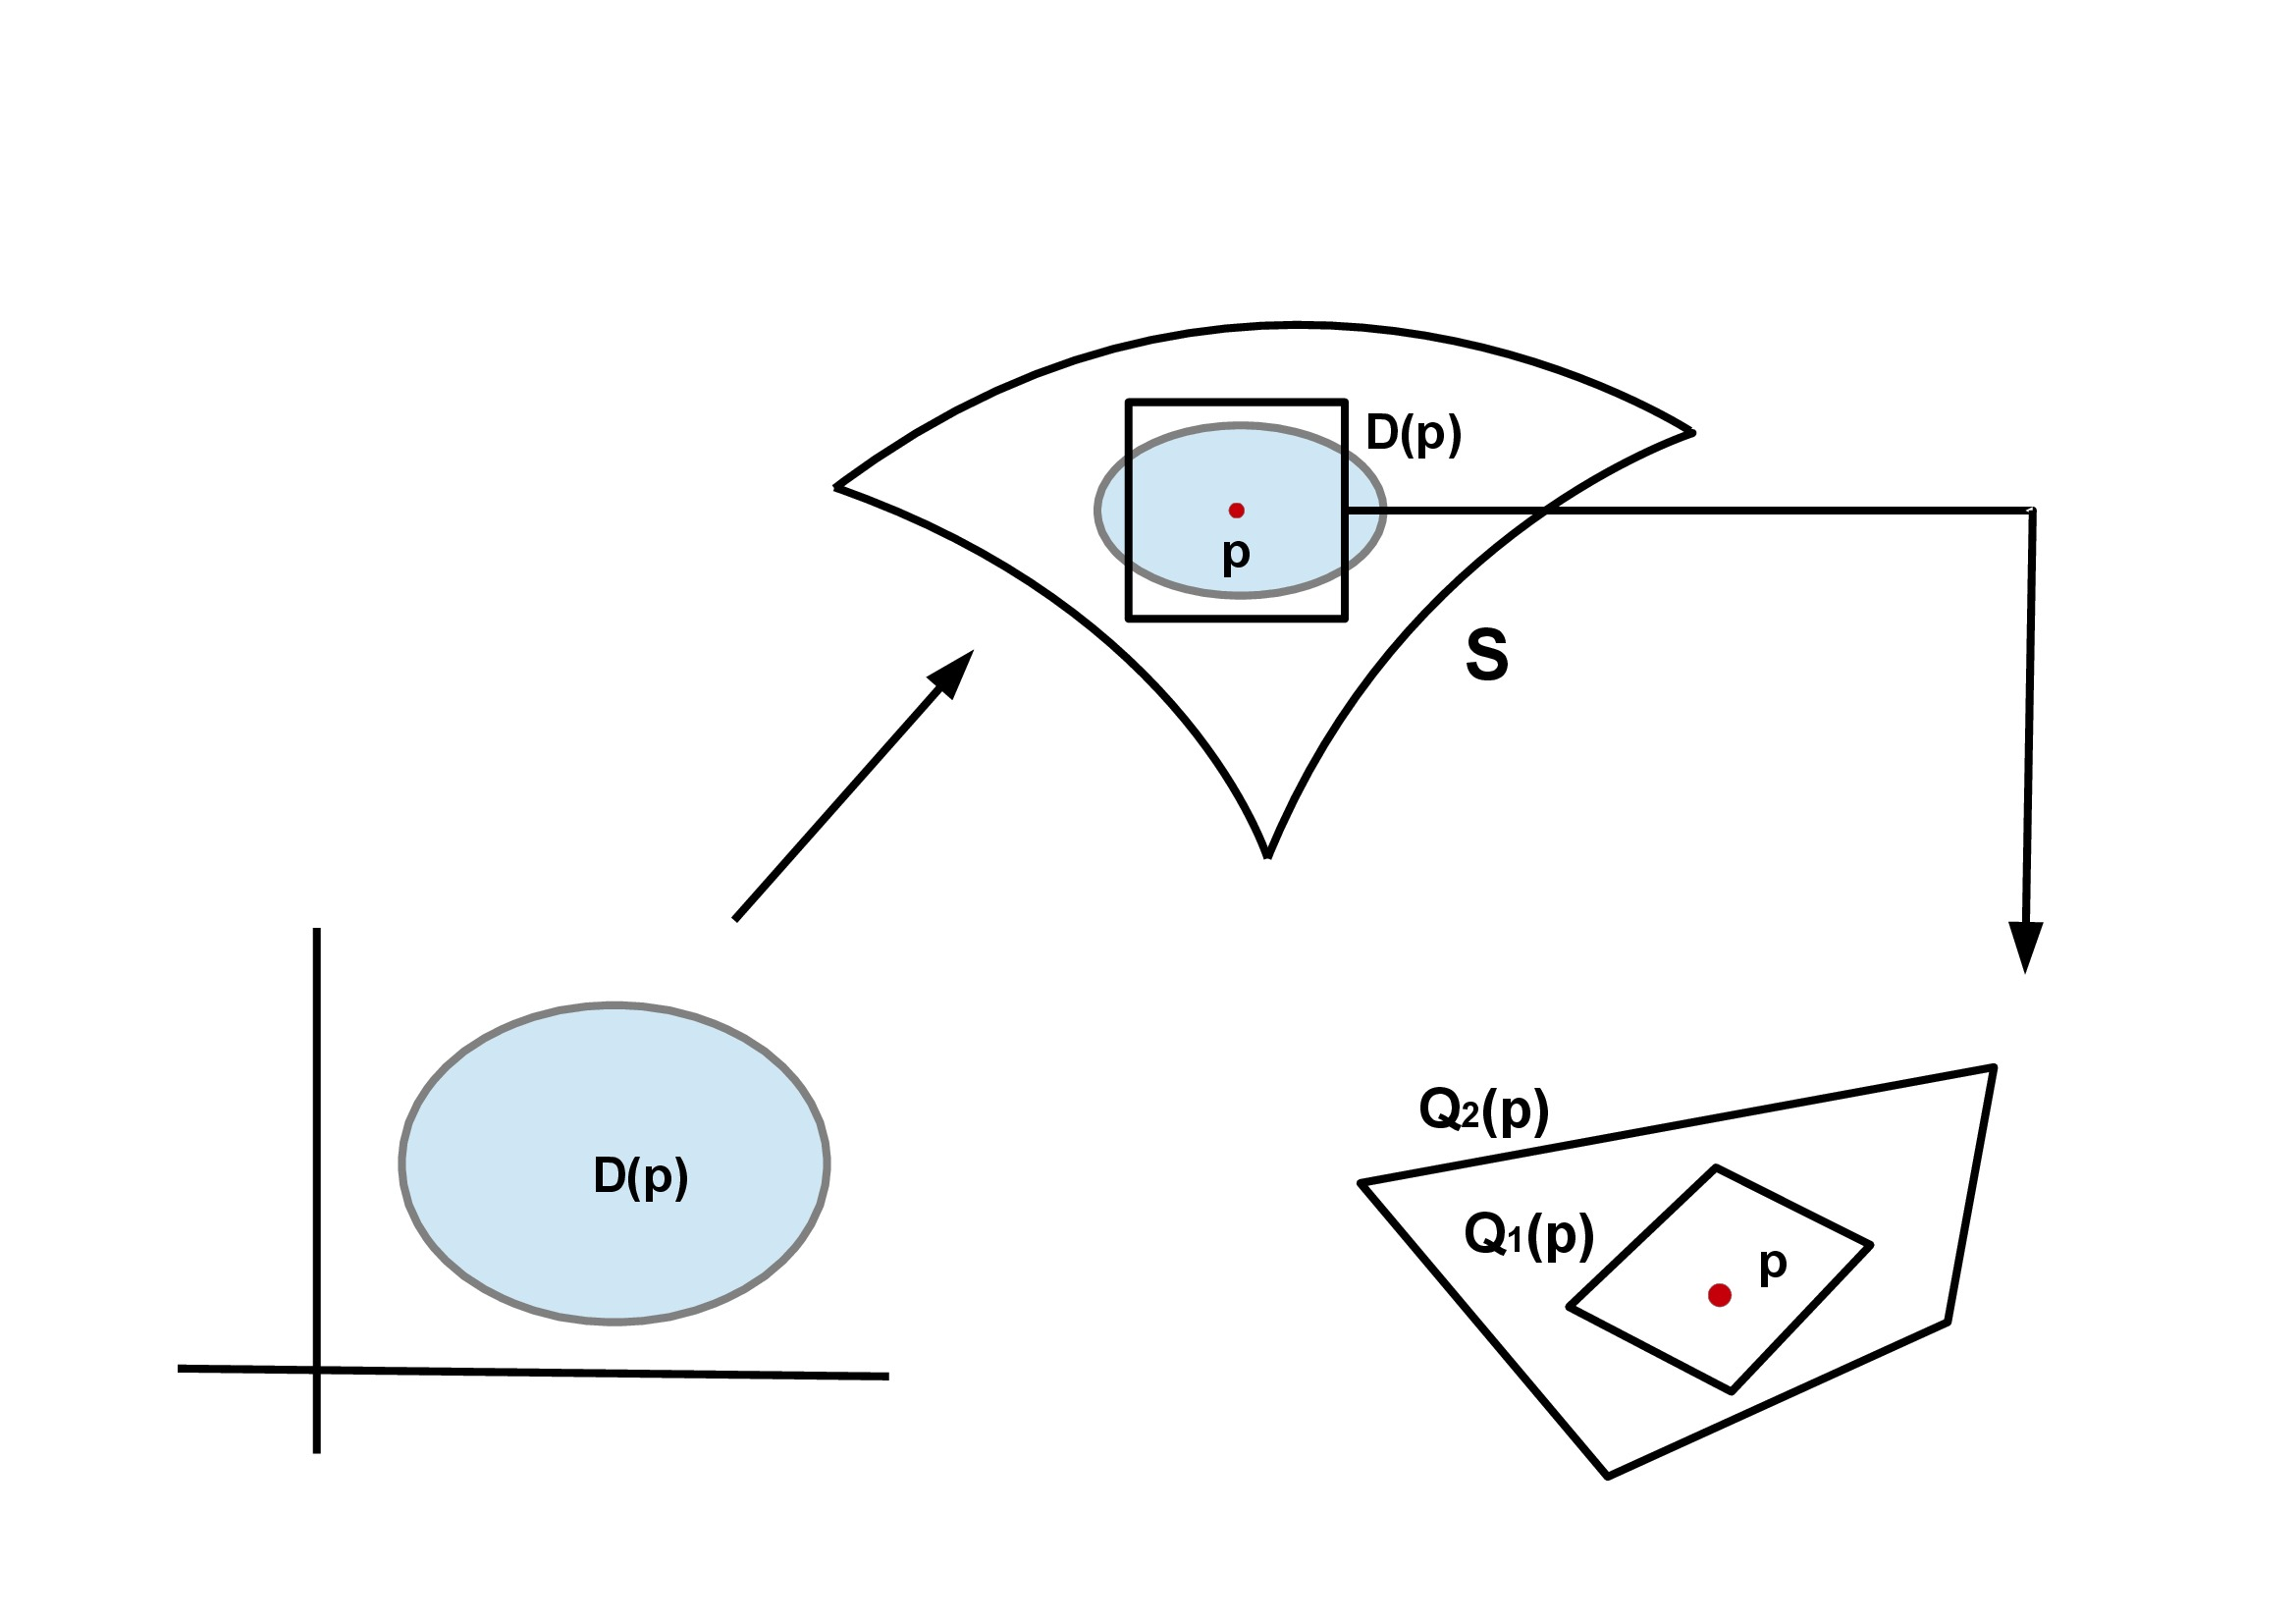
\includegraphics[width=10.0cm]{pic1.jpg}
\end{minipage}
\end{figure}

	Vistos como subconjuntos en el plano, $D(p_{1}),...,D(p_{n})$ se puede asumir que son disjuntos dos a dos (salvo trasladarlos convenientemente). A partir de aquí vamos a tomar estos subconjuntos fijos en el plano, teniendo siempre en cuenta que se corresponden con subconjuntos en $S$.

	Sin embargo, vamos a modificar el homeomorfismo entre $D(p_i)$ y su correspondiente conjunto en $S$ y considerar nuevos cuadrángulos $Q_{1}(p_i)$ de forma que $Q_{1}(p_{1}),...,Q_{1}(p_{n})$  determinen un embebimiento bicelular en S.

La clave será probar que existen cuadrados  $Q_{1}(p_{1}),...,Q_{1}(p_{n})$  como arriba, esto es con $Int(Q_{1}(p_j)) \subset Int(Q_{2}(p_j))\subset D(p_j)$ para todo $j$ y $S = \bigcup_{i = 1}^{n} Int(Q_{1}(p_{i}))$, de forma que  cada dos   tengan en común un número finito de puntos en común de $S$. 

\begin{figure}[h]
\centering
\begin{minipage}[c]{\textwidth}
\centering
    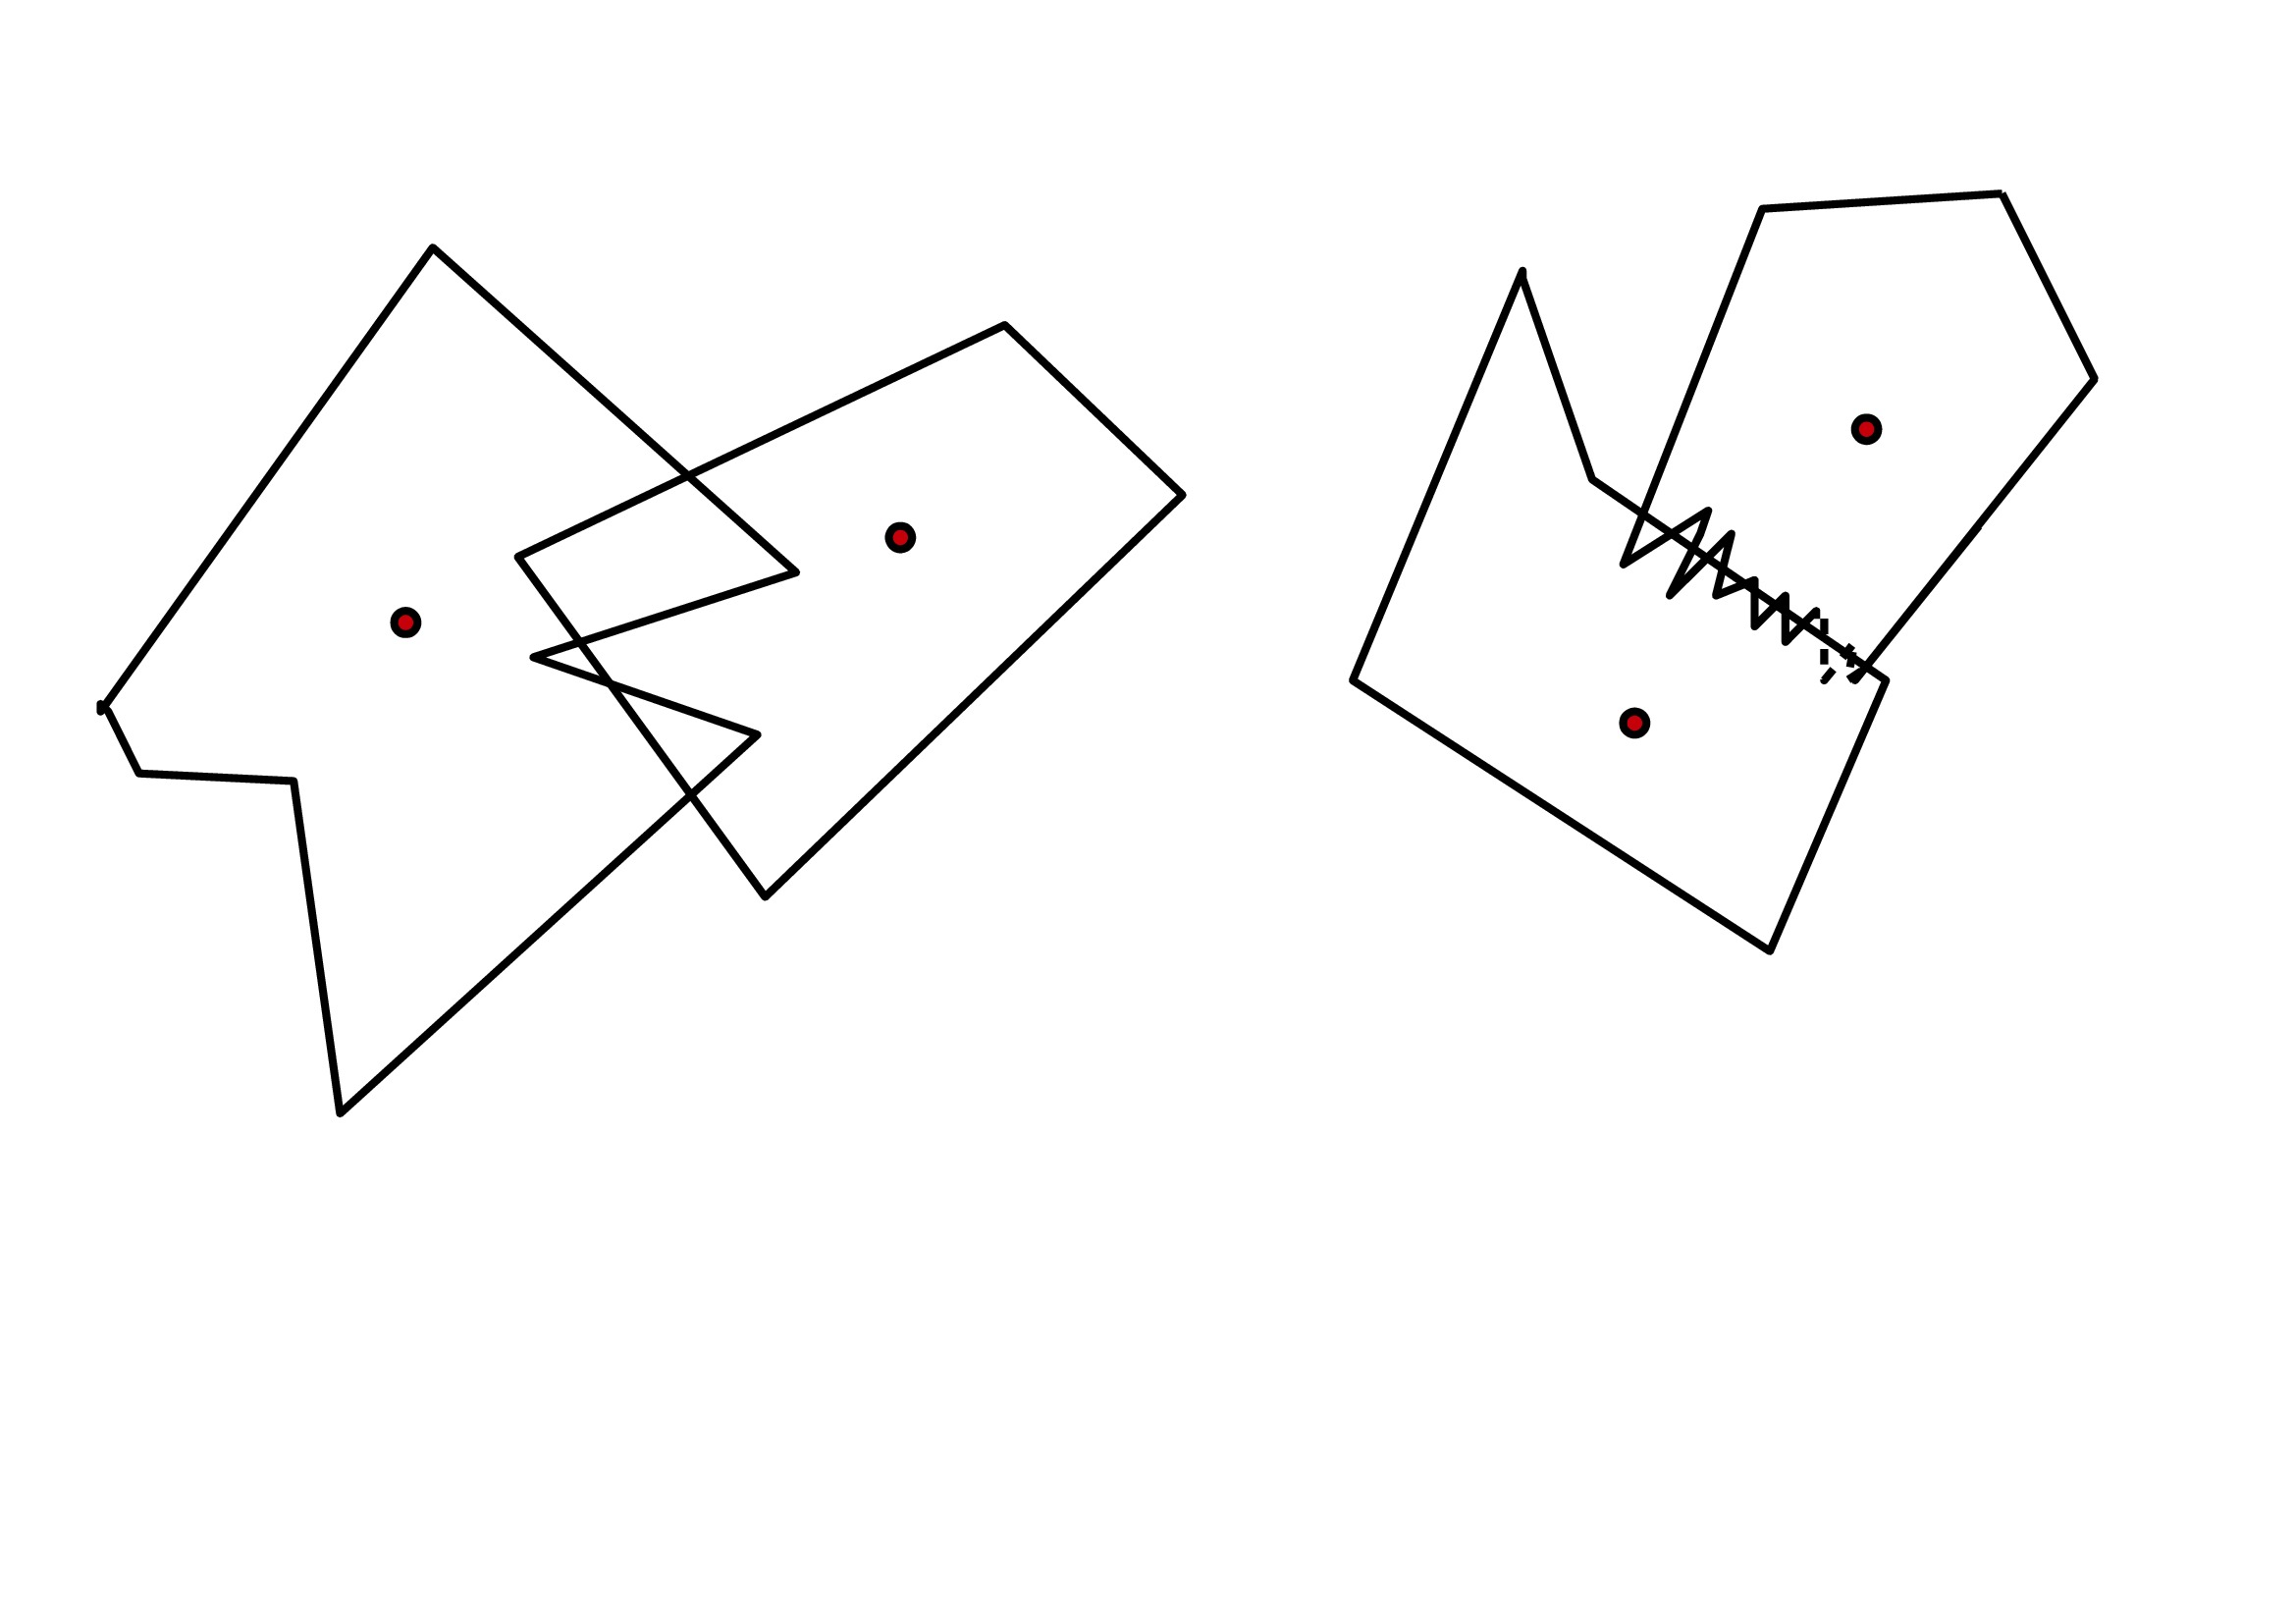
\includegraphics[width=10.0cm]{pic5.jpg}
\end{minipage}
\end{figure}

	Supongamos, por inducción sobre k, que los $Q_{1}(p_{1}),...,Q_{1}(p_{k-1})$ han sido escogidos de forma que cualquiera de cada dos tienen en común un número finito de puntos de $S$. 

	Ahora nos centramos en la posición relativa de los $Q_{1}(p_j)$ ($1 \leq j \leq k-1$) respecto a $Q_{2}(p_k)$. Un arco $P$ de algún $Q_{1}(p_j)$ ($1 \leq j \leq k-1$) que une dos puntos de $Q_{2}(p_k)$ y que tiene el resto de puntos en $Int(Q_{2}(p_k))$ se dirá un 
 {\em segmento malo}. 
 
Fijemos ahora $Q_{3}(p_k)$ un cuadrado entre $Q_{1}(p_k)$ y $Q_{2}(p_k)$. Diremos que  un segmento malo en $Q_{2}(p_k)$ es {\em muy malo} si interseca a $Q_{3}(p_k)$. Puede haber infinitos segmentos malos. Como los $Q_{1}(p_{j})$, $1\leq j\leq k-1$, son curvas de Jordan y por tanto homeomorfos a $\mathbb{S}^1$, no es difícil comprobar que sólo puede haber una cantidad finita de segmentos muy malos. Veámoslo:

\begin{figure}[h]
\centering
\begin{minipage}[c]{\textwidth}
\centering
    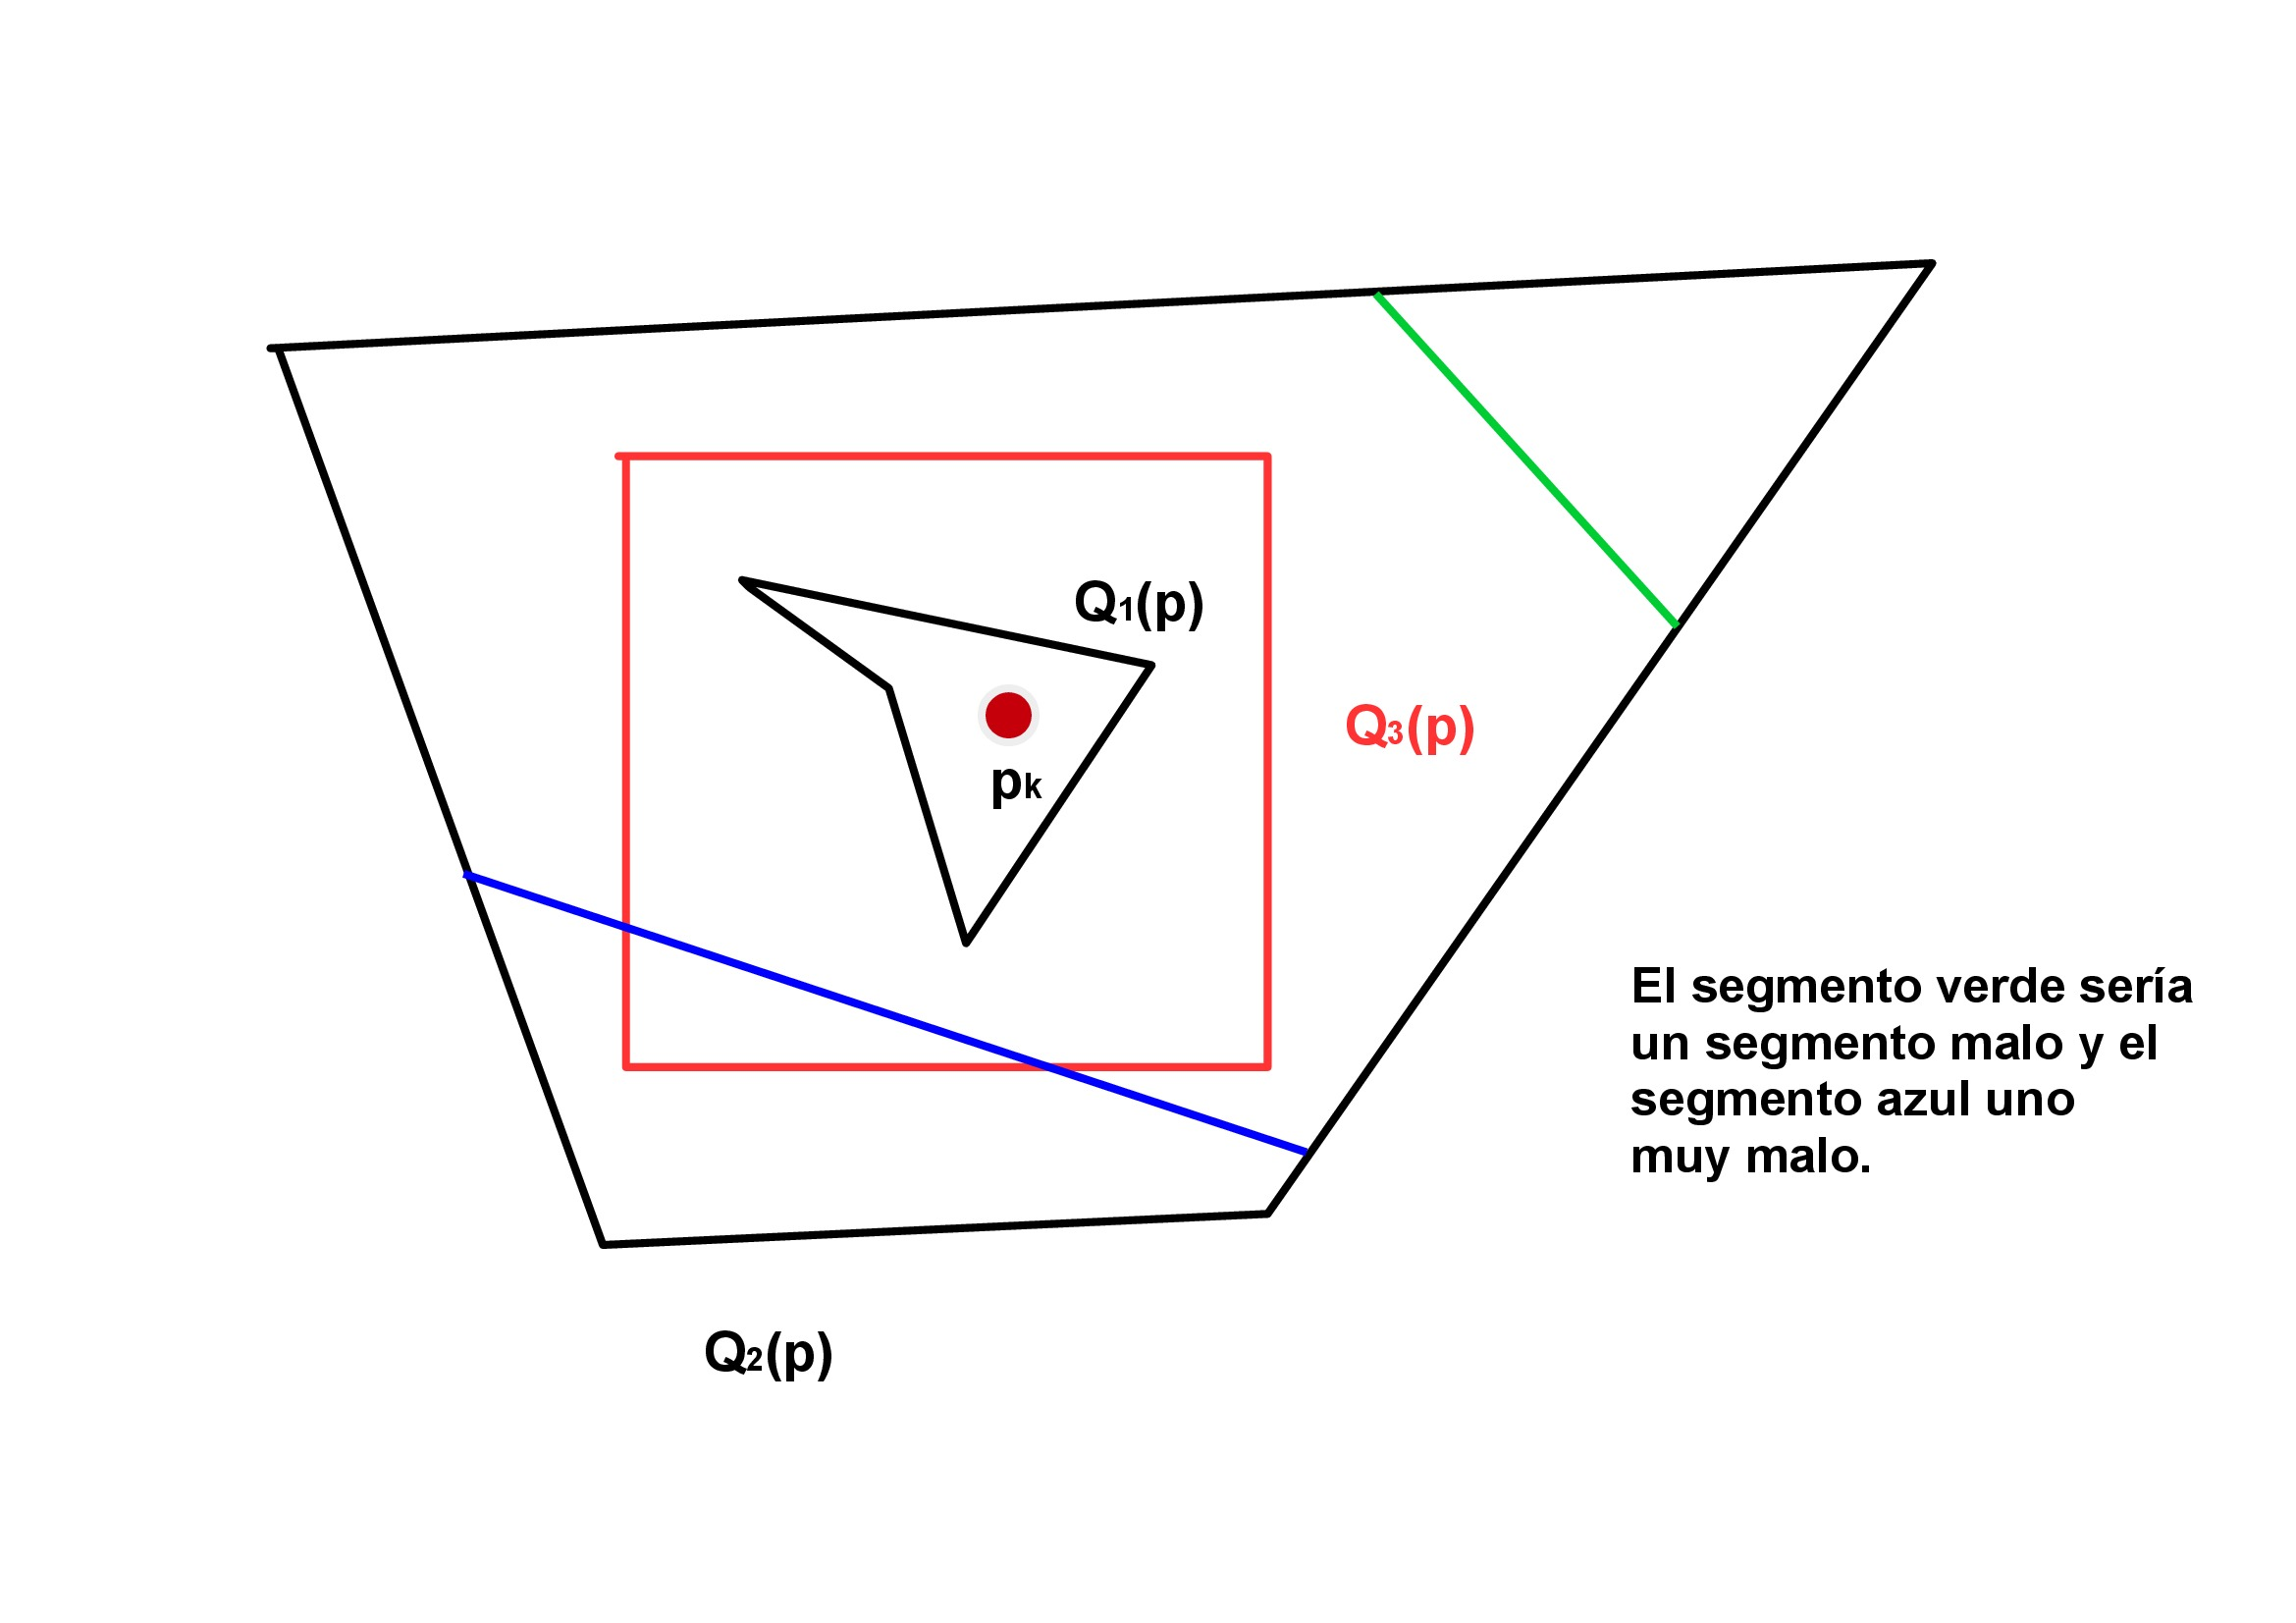
\includegraphics[width=10.0cm]{pic3.jpg}
\end{minipage}
\end{figure}

	Los segmentos muy malos junto con $Q_{2}(p_k)$ determinan un grafo biconexo $\Gamma$. Redibujemos $\Gamma$ dentro de $Q_{2}(p_k)$  para obtener un grafo $\Gamma'$ que sea plano-isomorfo a $\Gamma$ y tal que todas aristas de $\Gamma'$ son arcos poligonales simples. Técnicamente ésto se puede llevar a cabo gracias al lema \ref{lema27}, que si lo recordamos dice que un grafo biconexo puede ser obtenido a partir de un subgrafo biconexo de éste añadiendo caminos, sucesivamente, que unan dos vértices del grafo actual y que los otros vértices no estén en éste.

	Ahora aplicamos el teorema \ref{teorema33} para extender el plano-isomorfismo de de $\Gamma$ a $\Gamma'$ a un homeomorfismo de $\overline{Int(Q_{2}(p_k))}$ manteniendo $Q_{2}(p_k)$ fijado. Esto transforma $Q_{1}(p_k)$ y $Q_{3}(p_k)$ en curvas de Jordan $Q_{1}'$ y $Q_{3}'$ tales que $p_{k} \in Int(Q_{1}') \subset Int(Q_{3}')$.

	Consideremos una poligonal de Jordan $Q_{3}''$ en $Int(Q_{2}(p_k))$ tal que $Q_{1}' \subset Int(Q_{3}'')$ y además $Q_{3}''$ no interseca segmentos malos exceptuando los muy malos (que ahora son arcos poligonales simples).$^{1}$
	
\begin{figure}[h]
\centering
\begin{minipage}[c]{\textwidth}
\centering
    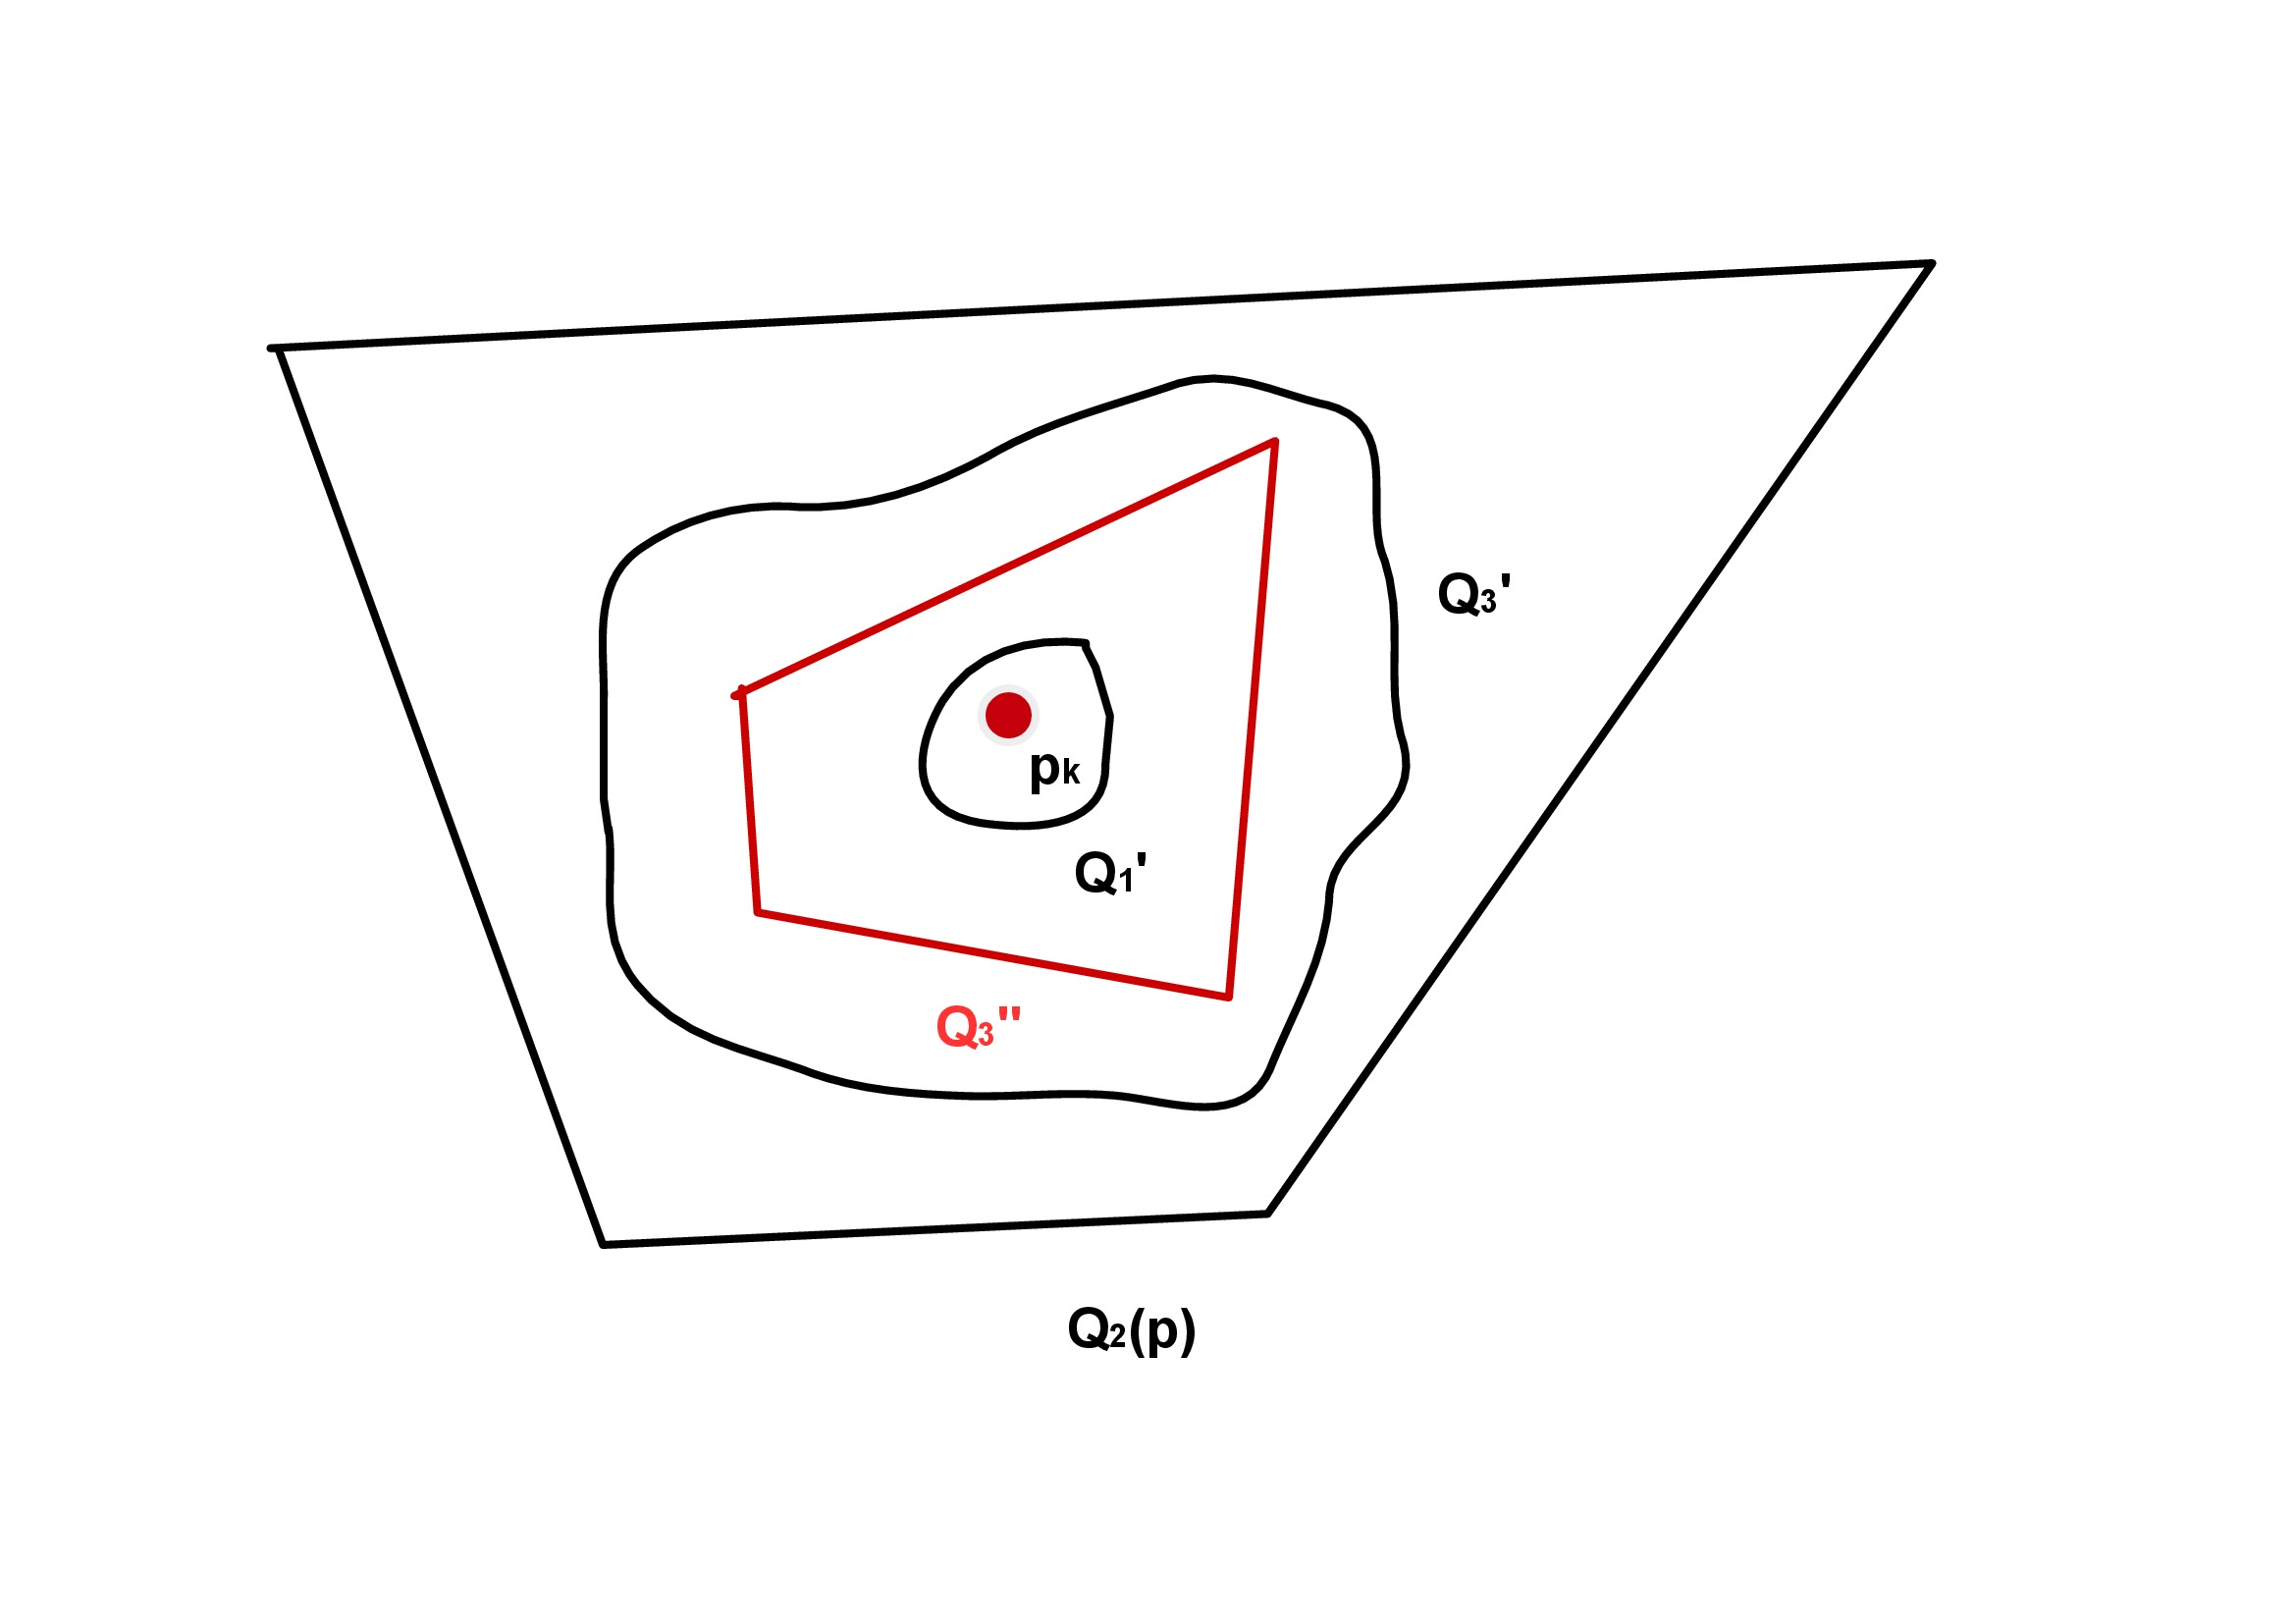
\includegraphics[width=10.0cm]{pic4.jpg}
\end{minipage}
\end{figure}
	
	Redibujando $\Gamma' \cup Q_{3}''$	(que es un grafo biconexo) y usando de nuevo el teorema \ref{teorema33} podemos asumir  que $Q_{3}''$ es un cuadrángulo con $Q_{1}'$ en su interior. Si ahora además elegimos $Q_{3}''$ como el nuevo $Q_{1}(p_k)$, entonces cualquiera de los $Q_{1}(p_1),..., Q_{1}(p_k)$ tiene intersecciones finitas dos a dos por ser finito el número de segmentos muy malos. Hemos cerrado la inducción.
 
	En consecuencia podemos asumir que que hay un número finito de segmentos muy malos dentro de cada $Q_{2}(p_k)$ y que además son arcos poligonales simples formando un grafo plano biconexo con $Q_{2}(p_k)$.

	La unión $\Delta:=\bigcup_{i = 1}^{n} Q_{1}(p_i)$ se puede ver como un grafo  en $S$ y cada región de $S \backslash \Delta$ está rodeada por un ciclo $C$ de $\Delta$. Ahora dibujamos un polígono convexo $C'$ de longitud 1 donde las esquinas de éste coincidan con los vértices de $\Delta$ en  $C$. Estos polígonos $C'$ se pueden suponer disjuntos dos a dos y conforman un subespacio $X'$ del plano. Identificando a pares los puntos de los lados de los polígonos en $X'$ con el criterio de {\em provenir del mismo punto} en una  arista de $\Delta$, el espacio identificación  $S'$ así obtenido es una superficie topológica, y el  grafo $\Delta'$ embebido bicelular asociado a esta identificación es naturalmente isomorfo a $\Delta$.

	Un isomorfismo de $\Delta$ a $\Delta'$ puede ser extendido a un homeomorfismo $f$ del conjunto de puntos de $\Delta$ en $S$ al conjunto de puntos de $\Delta'$ en $S'$. El teorema de Jordan-Schönflies nos permite extender $f$   a un homeomorfismo de $\overline{Int}(C)$ a $\overline{Int}(C')$ para cualesquiera celdas $C$ y $C'$, luego a un homeomorfismo de $S$ en $S'$. Esto prueba que $S$ es homeomorfa a una superficie triangulable, y concluye el teorema.
\end{proof}

	$^{1}$ La existencia de $Q_{3}''$ se puede establecer del siguiente modo: Para cada punto $p \in Q_{3}'$ definimos $R(p)$ un cuadrado que tiene a $p$ como punto medio y que además no corta los segmentos malos, excepto los que son muy malos. Consideramos entonces un recubrimiento finito de $Q_{3}'$ por cuadrados. La unión de estos cuadrados es un grafo plano biconexo cuyo ciclo exterior juega el papel de $Q_{3}''$.


\begin{remark} Como consecuencia directa del Teorema de Radó, toda superficie topológica compacta es homeomorfa a un polígono con lados identificados a pares. A partir de este hecho básico, y mediante métodos de cirugía topológica elemental, es posible demostrar que una superficie topológica compacta distinta de la esfera es homeomorfa a una suma conexa de toros o a una suma conexa de projectivos, siendo la unión de estas familias normalizadas de superficies exahustiva (esto es, no hay dos de ellas homeomorfas entre sí). Como corolario, toda superficie compacta se determina unívocamente por su característica de Euler y su carácter de orientabilidad; ver por ejemplo \cite{Massey}. Estos hechos forman parte del material abarcado por la asignatura Topología II del actual Grado en Matemáticas, por lo que no hemos considerado necesario redundar sobre ellos en este Trabajo Fin de Grado.
\end{remark}
